\documentclass[
]{jss}

%% recommended packages
\usepackage{orcidlink,thumbpdf,lmodern}

\usepackage[utf8]{inputenc}

\author{
Łukasz Chrostowski\\Adam Mickiewicz University \And Piotr
Chlebicki~\orcidlink{0009-0006-4867-7434}\\Stockholm University
\AND Maciej Beręsewicz~\orcidlink{0000-0002-8281-4301}\\Poznań
University of Economics and Business\\
Statistical Office in Poznań
}
\title{\pkg{nonprobsvy} -- An R package for modern methods for
non-probability surveys}

\Plainauthor{Łukasz Chrostowski, Piotr Chlebicki, Maciej Beręsewicz}
\Plaintitle{nonprobsvy -- An R package for modern methods for
non-probability surveys}
\Shorttitle{\pkg{nonprobsvy} for non-probability surveys}


\Abstract{
The paper presents \pkg{nonprobsvy} package which implements the
state-of-the-art statistical inference methods for non-probability
samples. The package implements various approaches that can be
categorized into three groups: prediction-based approach, inverse
probability weighting and doubly robust. On the contrary to the existing
packages \pkg{nonprobsvy} assumes existance of either full population or
probability-based population information and laverage the \pkg{survey}
package for the inference. The package implements both analytical and
bootstrap variance estimation for all of the proposed estimators. In the
paper we present the theory behind the package, its functionalities and
case study that showcases the usage of the package. The package is aimed
at official statisticans, public opinion or market researchers who
whould like to use non-probability samples to accurately estimate
popualtion characteristics.
}

\Keywords{data integration, doubly robust estimation, propensity score
estimation, mass
imputation, \proglang{R}, \proglang{Python}, \pkg{survey}}
\Plainkeywords{data integration, doubly robust estimation, propensity
score estimation, mass imputation, R, Python, survey}

%% publication information
%% \Volume{50}
%% \Issue{9}
%% \Month{June}
%% \Year{2012}
%% \Submitdate{}
%% \Acceptdate{2012-06-04}

\Address{
    Łukasz Chrostowski\\
    Pearson\\
    First line\\
Second line\\
  E-mail: \email{lukchr@st.amu.edu.pl}\\
  URL: \url{https://posit.co}\\~\\
      Piotr Chlebicki\\
    Stockholm University\\
    Matematiska institutionen\\
Albano hus 1\\
106 91 Stockholm, Sweden\\
  E-mail: \email{piotr.chlebicki@math.su.se}\\
  URL: \url{https://github.com/Kertoo},
\url{https://www.su.se/profiles/pich3772}\\~\\
      Maciej Beręsewicz\\
    Poznań University of Economics and Business\\
Statistical Office in Poznań\\
    \hfill\break
Poznań University of Economics and Business\\
Department of Statistics\\
Institute of Informatics and Quantitative Economics\\
Al. Niepodległosci 10\\
61-875 Poznań, Poland\\
\strut \\
Statistical Office in Poznań\\
ul. Wojska Polskiego 27/29\\
60-624 Poznań, Poland\\
  E-mail: \email{maciej.beresewicz@ue.poznan.pl}\\
  URL: \url{https://github.com/BERENZ},
\url{https://ue.poznan.pl/en/people/dr-maciej-beresewicz/}\\~\\
  }


% tightlist command for lists without linebreak
\providecommand{\tightlist}{%
  \setlength{\itemsep}{0pt}\setlength{\parskip}{0pt}}




\usepackage{amsmath, amsthm, amssymb} \usepackage{calc, ragged2e} \usepackage[ruled]{algorithm2e} \usepackage{algpseudocode} \newcommand{\argmin}{\operatornamewithlimits{arg\,min}} \newcommand{\argmax}{\operatornamewithlimits{arg\,max}} \newcommand{\bX}{\boldsymbol{X}} \newcommand{\bx}{\boldsymbol{x}} \newcommand{\bY}{\boldsymbol{Y}} \newcommand{\by}{\boldsymbol{y}} \newcommand{\bh}{\boldsymbol{h}} \newcommand{\bH}{\boldsymbol{H}} \newcommand{\ba}{\boldsymbol{a}} \newcommand{\bp}{\boldsymbol{p}} \newcommand{\bA}{\boldsymbol{A}} \newcommand{\bw}{\boldsymbol{w}} \newcommand{\bd}{\boldsymbol{d}} \newcommand{\bZ}{\boldsymbol{Z}} \newcommand{\bz}{\boldsymbol{z}} \newcommand{\bv}{\boldsymbol{v}} \newcommand{\bu}{\boldsymbol{u}} \newcommand{\bU}{\boldsymbol{U}} \newcommand{\bQ}{\boldsymbol{Q}} \newcommand{\bG}{\boldsymbol{G}} \newcommand{\HT}{\text{\rm HT}} \newcommand{\bbeta}{\boldsymbol{\beta}} \newcommand{\balpha}{\boldsymbol{\alpha}} \newcommand{\btau}{\boldsymbol{\tau}} \newcommand{\bgamma}{\boldsymbol{\gamma}} \newcommand{\btheta}{\boldsymbol{\theta}} \newcommand{\blambda}{\boldsymbol{\lambda}} \newcommand{\bPhi}{\boldsymbol{\Phi}} \newcommand{\bEta}{\boldsymbol{\eta}} \newcommand{\bZero}{\boldsymbol{0}} \newcommand{\colvec}{\operatorname{colvec}} \newcommand{\logit}{\operatorname{logit}} \newcommand{\Exp}{\operatorname{Exp}} \newcommand{\Ber}{\operatorname{Bernoulli}} \newcommand{\Uni}{\operatorname{Uniform}}

\begin{document}



\section{Introduction}\label{sec-introduction}

In official statistics, information about the target population and its
characteristics is mainly collected through probability surveys, census
or is obtained from administrative registers, which covers all (or
nearly all) units of the population. However, owing to increasing
non-response rates, particularly unit non-response and non-contact
(resulting from the growing respondent burden), as well as rising costs
of surveys conducted by National Statistical Institutes (NSIs),
non-probability data sources are becoming more popular
\citep{berkesewicz2017two, beaumont2020probability}. Non-probability
surveys, such as opt-in web panels, social media, scanner data, mobile
phone data or voluntary register data, are currently being explored for
use in the production of official statistics
\citep{citro2014multiple,daas2015big}, public opinion studies or market
research. Since the selection mechanism in these sources is unknown,
standard design-based inference methods cannot be directly applied.

To make it clear what we are dealing with we prepared Table
\ref{tab-comparison-characteristics} that compares the basic
characteristics of probability and non-probability samples. In
particular, what are the advantages and disadvantages of each type of
sample with respect to population coverage, bias, variance, costs, and
the selection mechanism for observations into the samples. In general,
non-probability samples suffers from unknown selection mechanism
(i.e.~unknown probabilities of inclusion into sample) and under-coverage
of certain groups from the population. As a result direct estimation
based on these samples are characterised with bias and, in most cases,
small variance (for large non-probability surveys) which leads to so
called big data paradox. Certainly, cost and timeliness of these surveys
is significantly smaller than for non-probability samples.

\begin{table}[ht!]
    \centering
    \begin{tabular}{lll}
    \hline
    \textbf{Factor}   &  \textbf{Probability sample} & \textbf{Non-probability sample}\\
    \hline
    Selection & Known probabilities & Unknown self-selection \\
    Coverage & Complete & Incomplete \\
    Estimation bias & Unbiased under design & Potential systematic bias \\
    Variance of estimates & Typically high & Typically low \\
    Cost & High & Low \\
    Availability & Long & Rapid \\
    \hline
    \end{tabular}
    \caption{Comparison of probability and non-probability samples and its characteristics}
    \label{tab-comparison-characteristics}
\end{table}

To address this problem, several approaches based on inverse probability
weighting (IPW), model-based prediction / mass imputation (MI) and
doubly robust (DR) estimators have been proposed for two main scenarios:
1) population-level data are available, either in the form of unit-level
data (e.g.~from a\textasciitilde register covering the whole population)
or known population totals/means, and 2) only survey data are available
as a\textasciitilde source of information about the target population
\citep[cf.][]{elliott_inference_2017}. \citet{wu2022statistical}
classified these approaches into three groups that require
a\textasciitilde joint randomization framework involving \(p\)
(probability sampling design) and one of the outcome regression model
\(\xi\) or propensity score model \(q\). In this approach the IPW
estimator is under the \(qp\) framework, the MI estimator is under the
\(\xi p\) framework, DR is under the \(qp\) or \(\xi p\) framework.

Most approaches assume that population data are used to reduce the bias
of non-probability sampling by a proper reweighting to reproduce known
population totals/means, by modelling \(E(Y|\boldsymbol{X})\) using
various techniques or combining both approaches (for instance doubly
robust estimators, cf.~\citet{chen2020doubly}; Multilevel Regression and
Post-stratification -- MRP also called \textit{Mister-P},
cf.~\citet{gelman1997poststratification}). Majority of these methods
rely on a limited number of moments of continuous or count data, with
some exceptions. For example, non-parametric approaches based on nearest
neighbours (NN), such as those discussed by Yang, Kim and Hwang
(\citeyear{yang2021integration}) or kernel density estimation (KDE)
described by Chen, Yang and Kim (\citeyear{chen_nonparametric_2022})
have also been proposed. It should be highlighted that, on contrary to
probability samples, there is no single method that can be used for
non-probability samples. Literature, and thus statistical software,
offers various methods as presented in the next section.

\subsection{Software for non-probability samples}\label{sec-software}

Table \ref{tab-comparisons} presents comparison of availability of
various inference methods and functionalities of selected packages. We
focused on packages available through CRAN or PyPI (for non-CRAN
packages see \citet{cobo2024software}). In the comparison we included
four packages that focuses on non-probability samples: \pkg{NonProbEst}
\citep{NonProbEst}, \pkg{balance} \citep{sarig2023balancepythonpackage},
\pkg{inps} \citep{castro2024inps} and our \pkg{nonprobsvy} as well as
two packages that implements specific, popular, methods: \pkg{rstanarm}
(Bayesian approach; MRP; \citet{rstanarm}) and \pkg{GJRM} (sample
selection models from econometrics; \citet{GJRM}). The \pkg{NonProbEst}
implements IPW under logistic regression as well as machine learning
approaches (e.g.~CART, GBM or Neural Networks) however does not provide
theoretical justification of using the ML approaches. The \pkg{balance}
focuses solely on the IPW and uses standard and covariate balancing
propensity score.

\begin{table}[ht!]
\centering
\resizebox{\linewidth}{!}{
\begin{tabular}{p{4cm}cccccc}
\hline
\textbf{Functionalities} & \pkg{NonProbEst} & \pkg{rstanarm} & \pkg{GJRM} & \pkg{balance} & \pkg{inps} & \pkg{nonprobsvy} \\
\hline
IPW  & $\checkmark$ & -- & +/- & $\checkmark$ & $\checkmark$ & $\checkmark$ \\
Calibrated IPW  & -- & -- & -- & -- & -- & $\checkmark$ \\
MI (population)   & $\checkmark$ & -- & -- & --& --& $\checkmark$ \\
MI (sample) & -- & -- & -- & -- & -- & $\checkmark$\\
DR & -- & -- & -- & -- & $\checkmark$ & $\checkmark$\\
MRP & -- & $\checkmark$ & -- & --  &--  & -- \\
Sample selection & -- & -- & $\checkmark$ & --  &--  & -- \\
Variable selection & -- & -- & -- & -- & -- & $\checkmark$\\
Analytical variance & -- & -- & -- & -- & -- & $\checkmark$\\
Bootstrap variance & +/- & -- & -- & & & $\checkmark$\\
Integration with \pkg{survey} or \pkg{samplics} & -- & -- & -- & -- & -- & $\checkmark$\\
\hline
\end{tabular}
}
\caption{Comparison of inference methods an of different packages}
\label{tab-comparisons}
\end{table}

It should be however noted that implementation of specific approaches
may vary significantly as the documentation of specific modules is
limited. For instance, \pkg{NonProbEst} allows for calibration of IPW
weights \textit{after} they are estimated, while \pkg{nonprobsvy} does
this in one step. On the other hand \pkg{NonProbEst} implements various
weights based on the estimated propensity scores while \pkg{nonprobsvy}
supports only two types of IPW weights. Furthermore, it should be noted
that \pkg{NonProbEst}, \pkg{balance} and \pkg{inps} implements survey
calibration for non-probability sample but it is not theoretically
justified as the inclusion probabilities are unknown (on the contrary to
probability samples).

In should be noted that only \pkg{nonprobsvy} leveraged the use of the
\pkg{survey} package to estimate analytic as well as bootstrap variance
of the non-probability estimators. Furthermore, none of the packages
focusing on frequentist approach to statistical inference implements
correct

This paper describes the nonprobsvy package for inference with
non--probability samples, available from the Comprehensive R Archive
Network (CRAN) at
\href{https://CRAN.R-project.org/package=nonprobsvy}{CRAN.R-project}.
Development version of the package can be also found at
\href{https://github.com/ncn-foreigners/nonprobsvy}{github}.

\section{Methods for non-probability
samples}\label{methods-for-non-probability-samples}

\subsection{Basic setup}\label{basic-setup}

Let \(U=\{1,..., N\}\) denote the target population consisting of \(N\)
labelled units. Each unit \(i\) has an associated vector of auxiliary
variables \(\boldsymbol{x}_{i}\) (a realisation of the random vector
\(\boldsymbol{X}_{i}\) in the super-population) and the study variable
\(y_{i}\) (a realisation of the random variable \(Y_{i}\) in the
super-population). Let \(\{ (y_i, \boldsymbol{x}_i), i \in S_A\}\) be a
dataset of a non-probability sample of size \(n_A\) and let
\(\{\left(\boldsymbol{x}_i, \pi_{i}\right), i \in S_B\}\) be a dataset
of a probability sample of size \(n_B\), where only information about
variables \(\boldsymbol{X}\) and inclusion probabilities \(\pi\) (which
in the super population model are also considered to be random
variables) are available. Let \(R_i\) be an indicator of inclusion into
non-probability sample. Each unit in the sample \(S_B\) has been
assigned a design-based weight given by \(d_i = 1/\pi_i\).

The goal is to estimate a finite population mean
\(\displaystyle\mu_{y}=\frac{1}{N}\sum_{i=1}^{N} y_{i}\) of the target
variable \(Y\). As values of \(y_{i}\) are not observed in the
probability sample, it cannot be used to estimate the target quantity.
Instead, one could try combining the non-probability and probability
samples to estimate \(\mu_{y}\). In this paper we do not consider
modifications for the possibly occurring overlap. The above description
of the data is presented in a more concise form in Table
\ref{tab-two-sources}.

\begin{table}[ht!]
    \centering
    \resizebox{\linewidth}{!}{
    \begin{tabular}{llccc} 
    \hline
    Sample & ID & Sample weight $d=\pi^{-1}$ & Covariates $\boldsymbol{x}$ & Study variable $y$ \\
    \hline
    Non-probability sample ($S_A$) & 1 & ? & $\checkmark$ & $\checkmark$ \\ 
    & $\vdots$ & ? & $\vdots$ & $\vdots$ \\
    & $n_A$ & ? & $\checkmark$ & $\checkmark$ \\
    Probability sample ($S_B$) & 1 & $\checkmark$ & $\checkmark$ & ? \\
    & $\vdots$ & $\vdots$ & $\vdots$ & ? \\ 
    & $n_B$ & $\checkmark$ & $\checkmark$ & ? \\                                     
    \hline     
    \end{tabular}
    }
    \caption{Two sample setting.}
    \label{tab-two-sources}
\end{table}

\subsection{Prediction-based approach}\label{prediction-based-approach}

\subsubsection{Mass imputation}\label{mass-imputation}

Imputation refers to the process of replacing missing or incomplete data
with substituted values. The goal of imputation is to allow for more
complete data analysis, as many statistical methods require complete
datasets.

Mass imputation is the application of imputation techniques to an entire
dataset where many observations have missing values for the given
variable. \cite{kim_combining_2021}, \cite{yang2021integration},
\cite{Beres} propose the following imputation strategies as:

\begin{itemize}
    \item Model based approach (GLM),
    \item Nearest neigbour imputation (NN),
    \item Predictive mean mathing (PMM).
\end{itemize}

Mass imputation is particularly useful in large datasets where missing
data can be widespread, and it seeks to preserve the relationships
between variables, thus improving the overall integrity of the data.

As presented in (Table \ref{tab-two-sources}), we do not know the value
of the dependent variable \(Y\) for the units in the probability sample.
In this case, the method will be to impute the values of the explanatory
variable for all units in the probability sample. We therefore treat the
non-probability sample as a training set that is used to build the
imputation model. In this subsection, we distinguish three main methods
of mass imputation based on linear models and the k-nearest neighbours
algorithm. Other popular methods for estimating the variable \(Y\) from
the variable \(\boldsymbol{X}\) can also be considered, e.g.~machine
learning models such as random forests or neural networks.

We can obtain an estimate of the population mean based on known design
weights and an imputation model for units from the probability sample:

\begin{equation}
\hat{\mu}_{M I}=\frac{1}{\hat{N}_{\mathrm{B}}} \sum_{i \in S_{\mathrm{B}}} d_i^{\mathrm{B}} \hat{y}, 
\end{equation} \(\hat{N}_{\mathrm{B}} = \sum_{i \in S_B} d_i^B\) and
\(\hat{y}\) is the estimated value of \(y\) for units from probability
samples based on mass imputation model.

This estimator can be understood as a version of the Horvitz--Thompson
estimator, which are used to estimate mean or total values in the
population (based on probability sampling and inclusion probabilities).
The only difference is that in our case, instead of the known values of
the \(Y\) variable, we use its estimated equivalents.

\subsubsection{Generalized Linear
Models}\label{generalized-linear-models}

Let us assume the following parametric model for the sample \(S_A\)
based on the conditional expected value of the variable \(Y\). Let
\begin{equation}
\mathbb{E}\left(y_i \mid \boldsymbol{x}_i\right)=m\left(\boldsymbol{x}_i, \boldsymbol{\beta}_0\right)
\end{equation} for a certain \(p\)--dimensional vector
\(\boldsymbol{\beta}_0\) and a known \(m\) function from a given class
of mean functions for generalized linear models.

According to the model described, we have \[
y_i=m\left(\boldsymbol{x}_i\right)+\varepsilon_i, \quad i=1,2, \ldots, N.
\] We also assume that the random variables \(\varepsilon_i\) are
independent with \(\mathbb{E} \left(\varepsilon_i \right) = 0\) and
\(\sigma^2 \left(\varepsilon_i \right) = \mathbf{v} \left(\boldsymbol{x}\right) \sigma^2\).
It is assumed that \(\mathbf{v} \left(\boldsymbol{x}\right)\) has a
known value and is homogeneous, i.e.~homogeneous, regardless of the
sample under study. Let us represent the process of mass imputation of a
linear model to a sample \(S_B\). Finally we are interested in finding a
vector \(\boldsymbol{\beta}\) solves the following equation:
\begin{equation}
\label{eq-2.3}
U(\boldsymbol{\beta})=\frac{1}{n_A} \sum_{i \in S_A}\left\{y_i-m\left(\boldsymbol{x}_i ; \boldsymbol{\beta}\right)\right\} h\left(\boldsymbol{x}_i ; \boldsymbol{\beta}\right)=\mathbf{0},
\end{equation}

for some \(p\)-dimensional vector of function
\(h\left(\boldsymbol{x}_i ; \boldsymbol{\beta}\right)\), where
\(h\left(\boldsymbol{x}_i ; \boldsymbol{\beta}\right) = \boldsymbol{x}_i\)
might be used for certain applications. The mass imputation process is
described in Algorithm \ref{algo-1}.

\subsubsection{Nearest Neighbour
Algorithm}\label{nearest-neighbour-algorithm}

On the other hand, it is also possible to consider a non-parametric
model for the problem described, i.e.~for each individual from sample
\(S_B\), the k-nearest neighbours from sample \(S_A\) are found based on
the values of the auxiliary vector \(\boldsymbol{X}\) and the
corresponding metric. Then, the missing values of the variable \(Y\)
from sample \(S_B\) are replaced by the values (or their mean if more
than one neighbour is considered) of this variable for the corresponding
neighbours from sample \(S_A\). The algorithm is as follows

Note that the algorithm differs depending on the number of nearest
neighbours chosen. In case \(k=1\) the nearest neighbour value is
imputed according to the chosen metric, for example the Euclidean
metric. In case \(k>2\) the average of the nearest neighbours values is
imputed. The literature indicates that this method suffers from the
so-called curse of multidimensionality, i.e.~for samples with several
explanatory variables, imputation can lead to a large variance in the
estimator. On the other hand, the algorithm is easy to interpret and
simple to implement.

\subsubsection{Predictive Mean Matching}\label{predictive-mean-matching}

Predictive mean-matching imputation is a particularly well-known way of
dealing with non-response among respondents, and is favoured by
statistical offices for compiling a country's official population
statistics. It is a version of the k-nearest neighbour algorithm, but
instead of looking at the distances between the vectors of the auxiliary
variables, it looks at the distance between the functions of the mean
vectors. This helps to reduce the curse of multidimensionality and, at
the same time, allows the observed values of the explanatory variable or
their mean to be calculated. Let us therefore present two algorithms
that describe the steps to follow to perform a mass imputation using the
mean matching method.

As can be seen, the difference between the two algorithms is due to step
2. In the first approach, we compare \(\hat{y}\) from samples \(S_A\)
and \(S_B\). The second, on the other hand, compares \(\hat{y}\) from
sample \(S_B\) with the known \(y\) from sample \(S_A\). It is worth
noting that proof of the consistency of these estimators can be found in
\citet{Beres}.

\subsection{Inverse Probability Weighting}\label{sec-ipw}

The main disadvantage of non-probability sampling is the unknown
selection mechanism for a unit to be included in the sample. This is why
we talk about the so-called biased sample problem. The inverse
probability approach is based on the assumption that a reference
probability sample is available and therefore we can estimate the
propensity score of the selection mechanism. In recent years, a number
of articles have addressed this issue. \cite{chen2020doubly} propose
maximum likelihood estimation approach for estimating propensity scores
for selection mechanism. \cite{wu2022statistical} present the approach
based on generalized estimating equations, this method is also mentioned
in \cite{yang_doubly_2020}. On the other hand calibration approach for
quantiles was explained \cite{beresewicz2024inference} and
\cite{santanna_covariate_2022} present the approach based on maximize
the covariate distribution balance among different treatment groups.

In the formal framework, let us introduce the following assumptions for
propensity score model, which will imply a number of properties derived
in the thesis.

\begin{itemize}
    \item[(A1)] The selection indicator $R_i^A$ and explanatory variable $y_i$ are independent.
    \item[(A2)]All units have a so-called non-probability sample propensity score, which is non-zero, i.e. $\pi_i^{\mathrm{A}} > 0$, where $\pi_i^{\mathrm{A}} = P_q\left(R_i^A=1 \mid \boldsymbol{x}_i, y_i\right)$, where $q$ refers to the model for the selection mechanism for the non-probability sample (propensity score model).
    \item[(A3)] Indicator variables $R_i^A$ and $R_j^A$ are independent with $i \neq j$. 
\end{itemize}

The estimated propensity score is used to construct an inverse
probability weighting estimator of the population mean of the form

\begin{equation}
\begin{gathered}
\hat{\mu}_{I P W}=\frac{1}{\hat{N}^A} \sum_{i \in S_A} \frac{y_i}{\hat{\pi}_i^A}.
\end{gathered}
\end{equation} where
\(\hat{N}^A = \sum_{i \in S_A} \hat{d}_i^A = \sum_{i \in S_A} \frac{1}{\hat{\pi}_i^A}\).

\subsubsection{Maximum Likelihood
Estimation}\label{maximum-likelihood-estimation}

Consider the following likelihood function \begin{align}
    \begin{split}
 \ell(\boldsymbol{\theta}) & =\sum_{i=1}^N\left\{R_i^A \log \pi_i^{\mathrm{A}}+\left(1-R_i^A\right) \log \left(1-\pi_i^{\mathrm{A}}\right)\right\} \\ & =\sum_{i \in S_{\mathrm{A}}} \log \left\{\frac{\pi\left(\boldsymbol{x}_i, \boldsymbol{\theta}\right)}{1-\pi\left(\boldsymbol{x}_i, \boldsymbol{\theta}\right)}\right\}+\sum_{i=1}^N \log \left\{1-\pi\left(\boldsymbol{x}_i, \boldsymbol{\theta}\right)\right\}
    \end{split}
\end{align} In practice, a function of this form cannot be used because
we do not observe all units from the population. Hence, the second
component of the function is replaced by the Horvitz-Thompson estimator,
which is used when having access to the design weights for the units in
the sample. In our case, these will be the weights \(d_i^B\) for the
units in the sample \(S_B\). We then have \begin{equation}
\ell^*(\boldsymbol{\theta})=\sum_{i \in S_{\mathrm{A}}} \log \left\{\frac{\pi\left(\boldsymbol{x}_i, \boldsymbol{\theta}\right)}{1-\pi\left(\boldsymbol{x}_i, \boldsymbol{\theta}\right)}\right\}+\sum_{i \in S_{\mathrm{B}}} d_i^{\mathrm{B}} \log \left\{1-\pi\left(\boldsymbol{x}_i, \boldsymbol{\theta}\right)\right\}.
\end{equation} Our objective is to find the maximum likelihood estimator
\(\hat{\pi}_{i}^{A} = \pi(\boldsymbol{x}_{i}, \hat{\boldsymbol{\theta}})\),
such that \(\hat{\boldsymbol{\theta}}\) maximises the function defined
above.

\subsubsection{Generalized Estimating Equations}\label{sec-ipw-gee}

Equations of the type
\(\operatorname{U}(\boldsymbol{\theta}) = \boldsymbol{0}\), where
\(\operatorname{U}(\boldsymbol{\theta}) = \frac{\partial}{\partial \boldsymbol{\theta}} l^*(\boldsymbol{\theta})\),
obtained from the maximum likelihood estimation can be replaced by a
system of generalized estimating equations of the form \begin{equation}
\label{gee}
\mathbf{G}(\boldsymbol{\theta})=\sum_{i \in S_A} h\left(\boldsymbol{x}_i, \boldsymbol{\theta}\right)-\sum_{i \in S_B} d_i^B \pi\left(\boldsymbol{x}_i, \boldsymbol{\theta}\right) h\left(\boldsymbol{x}_i, \boldsymbol{\theta}\right) = \boldsymbol{0},
\end{equation} where
\(h\left(\boldsymbol{x}_i, \boldsymbol{\theta}\right)\) is a certain
continuous function. In the literature, the most commonly considered
functions are
\(h\left(\boldsymbol{x}_i, \boldsymbol{\theta}\right) = \boldsymbol{x}_i\)
and
\(h\left(\boldsymbol{x}_i, \boldsymbol{\theta}\right) = \boldsymbol{x}_i \pi\left(\boldsymbol{x}_i, \boldsymbol{\theta}\right)^{-1}\).
Note that if the function \(h\) is equal to the vector of observed
characteristics \(\boldsymbol{x}\), then \(\mathbf{G}\) is reduced to \[
\mathbf{G}(\boldsymbol{\theta}) = \sum_{i \in S_A} \boldsymbol{x}_i-\sum_{i \in S_B} d_i^B \pi\left(\boldsymbol{x}_i, \boldsymbol{\theta}\right) \boldsymbol{x}_i.
\] In the next subsection we will proof that this is disorted version of
MLE approach with \(\pi_i^A\) modelling by logistic regression. If we
use the second form of the function \(h\) we get the following form of
the function \(\mathbf{G}\) \[
\mathbf{G}(\boldsymbol{\theta}) = \sum_{i \in S_A} \frac{\boldsymbol{x}_i}{\pi\left(\boldsymbol{x}_i, \boldsymbol{\theta}\right) }-\sum_{i \in S_B} d_i^B \boldsymbol{x}_i.
\]

The advantage of this method is the ability to estimate with global
values of the variables (e.g.~from external sources) instead of a
probability sample. Note that this is allowed by the second form of the
\(\mathbf{G}\) function. Its second term is nothing more than the
estimated sums of the \(\boldsymbol{x}\) variables. On the other hand,
empirical studies suggest that the process of solving this type of
equation may be less stable than the maximum likelihood method. In other
words, the iterative algorithm for finding zeros that satisfy equation
(\ref{gee}) may not converge.

In the \texttt{nonprobsvy} package the propensity scores can modelled
using three different link functions: logistic, complementary log-log
and probit. The logistic regression is the most commonly used for
modelling probabilities. This method is based on the so-called sigmoidal
function and for our settign it has the form It satisfies certain
properties to model the probability. For our scheme, this will be the
probability of belonging to the non-probability sample. Another approach
to modelling binary variables and also probabilities is probit
regression. It is based on the standard normal distribution and as logit
is also symmetric around \(p = 0.5\). On the other hand regression with
the cloglog model is particularly useful if we are modelling rare
phenomena, i.e.~the probabilities will oscillate around the values 1 and
0. Compared to the sigmoidal function and the distribution, the cloglog
function is more asymmetric towards the value 0.5.

\subsection{Doubly Robust approach}\label{doubly-robust-approach}

The inverse probability weighting and mass imputation estimators are
sensible on misspecified models for propensity score and outcome
variable respectively. For this purpose so called doubly-robust methods,
which take into account these problems, are presented.

The proposed estimation procedure addresses the challenge of combining
data from nonprobability and probability survey samples. Traditional
semiparametric models, often applied to such problems, are not directly
usable in this context due to the distinct nature of the two samples.
Instead, a joint randomization framework is employed, integrating
semiparametric models for propensity scores with outcome regression for
the nonprobability sample and design-based inference from the
probability sample. This framework leads to a doubly robust (DR)
estimation approach, which is effective in the presence of model
misspecifications.

Inverse Probability Weighted (IPW) estimators are sensitive to
misspecified propensity score models, particularly when propensity
scores are very small. To improve robustness and efficiency, the doubly
robust method incorporates a prediction model for the response variable.
Moreover, even if one of the models is misspecified, the DR estimator
remains consistent, showcasing the ``double robustness'\,' property.

\subsubsection{Joint Randomization
Approach}\label{joint-randomization-approach}

The joint randomization approach combines two processes: the selection
mechanism of a non-probability sample, modelled by propensity scores,
and the design-based inference from a probability sample.

The response \(y_i\) is predicted using a regression model
\(m(\boldsymbol{x}_i, \boldsymbol{\beta})\) (or NN/PMM methods), where
\(\boldsymbol{\beta}\) is estimated from the non-probability sample.
With known design weights \(d_i^B\) for \(i \in S_B\) we can define the
DR estimator as \begin{equation}
\label{dr}
\hat{\mu}_{\mathrm{DR}}=\frac{1}{\hat{N}^{\mathrm{A}}} \sum_{i \in S_{\mathrm{A}}} d_i^{\mathrm{A}}\left\{y_i-m\left(\boldsymbol{x}_i, \hat{\boldsymbol{\beta}}\right)\right\}+\frac{1}{\hat{N}^{\mathrm{B}}} \sum_{i \in S_{\mathrm{B}}} d_i^{\mathrm{B}} m\left(\boldsymbol{x}_i, \hat{\boldsymbol{\beta}}\right),
\end{equation} where
\(d_i^A=\pi\left(\boldsymbol{x}_i, \boldsymbol{\theta}\right)^{-1}, \hat{N}^A=\sum_{i \in S_A} d_i^A\)
and \(\hat{N}^B=\sum_{i \in S_B} d_i^B\).

It remains consistent if either the propensity score model
\(\pi(\boldsymbol{x}_i, \boldsymbol{\theta})\) or the outcome regression
model \(m(\boldsymbol{x}_i, \boldsymbol{\beta})\) is correctly
specified.

The joint randomization approach ensures robustness by accounting for
randomness in both the non-probability sample through
\(\pi(\boldsymbol{x}_i, \boldsymbol{\theta})\) and the probability
sample through design-based inference.

\subsubsection{Minimization of the bias for doubly robust
methods}\label{minimization-of-the-bias-for-doubly-robust-methods}

By reducing the variance of the estimators, for example by variable
selection, we cannot control the bias of the estimator, which may
increase. Therefore, according to \citet{yang_doubly_2020}, the idea is
to determine the equations leading to the estimation of the
\(\boldsymbol{\beta}\) and \(\boldsymbol{\theta}\) parameters based on
the bias of the population mean estimator. In contrast to the joint
randomization approach, this method allows for the estimation of the
parameters \(\boldsymbol{\beta}\) and \(\boldsymbol{\theta}\) in a
single step, rather than in two separate steps.

We will first present the bias of the doubly robust estimator and then,
using optimisation techniques, discuss the equations leading to its
minimization. Thus we have \begin{equation}
\begin{aligned}
\operatorname{bias}\left(\hat{\mu}_{D R}\right) & = \mid\hat{\mu}_{DR}-\mu\mid& \\
& =\frac{1}{N} \sum_{i=1}^N\left\{\frac{R_i^A}{\pi_i^A\left(\boldsymbol{x}_i^{\mathrm{T}} \boldsymbol{\theta}\right)}-1\right\}\left\{y_i-m\left(\boldsymbol{x}_i^{\mathrm{T}} \boldsymbol{\beta}\right)\right\}\\
& + \frac{1}{N} \sum_{i=1}^N\left(R_i^B d_i^B-1\right) m\left(\boldsymbol{x}_i^{\mathrm{T}} \boldsymbol{\beta}\right)
\end{aligned}
\end{equation}

To minimize \(\operatorname{bias}\left(\hat{\mu}_{D R}\right)^2\) let us
calculate the gradient of the square of the bias at
\(\left(\boldsymbol{\beta}, \boldsymbol{\theta}\right)\). We then have

\begin{equation*}
\frac{\partial \operatorname{bias}\left(\hat{\mu}_{D R}\right)^2}{\partial\left(\boldsymbol{\beta}^{\mathrm{T}}, \boldsymbol{\theta}^{\mathrm{T}}\right)^{\mathrm{T}}}=2 \operatorname{bias}\left(\hat{\mu}_{D R}\right) J(\theta, \beta),
\end{equation*} where \begin{equation*}
J(\theta, \beta)=\left(\begin{array}{l}
J_1(\theta, \beta) \\
J_2(\theta, \beta)
\end{array}\right)=\left(\begin{array}{c}
\sum_{i=1}^N R_i^A\left\{\frac{1}{\pi\left(\boldsymbol{x}_i, \boldsymbol{\theta}\right)}-1\right\}\left\{y_i-m\left(\boldsymbol{x}_i, \boldsymbol{\beta}\right)\right\} \boldsymbol{x}_i \\
\sum_{i=1}^N \frac{R_i^A}{\pi\left(\boldsymbol{x}_i, \boldsymbol{\theta}\right)} \frac{\partial m\left(\boldsymbol{x}_i, \boldsymbol{\beta}\right)}{\partial \boldsymbol{\beta}}-\sum_{i \in S_{\mathrm{B}}} d_i^{\mathrm{B}} \frac{\partial m\left(\boldsymbol{x}_i, \boldsymbol{\beta}\right)}{\partial \boldsymbol{\beta}}
\end{array}\right),
\end{equation*} which leads to the problem of solving the following
system of equations \begin{equation}
\label{bias-min}
    \left(\begin{array}{c}
\sum_{i=1}^N R_i^A\left\{\frac{1}{\pi\left(\boldsymbol{x}_i, \boldsymbol{\theta}\right)}-1\right\}\left\{y_i-m\left(\boldsymbol{x}_i, \boldsymbol{\beta}\right)\right\} \boldsymbol{x}_i \\
\sum_{i=1}^N \frac{R_i^A}{\pi\left(\boldsymbol{x}_i, \boldsymbol{\theta}\right)} \frac{\partial m\left(\boldsymbol{x}_i, \boldsymbol{\beta}\right)}{\partial \boldsymbol{\beta}}-\sum_{i \in S_{\mathrm{B}}} d_i^{\mathrm{B}} \frac{\partial m\left(\boldsymbol{x}_i, \boldsymbol{\beta}\right)}{\partial \boldsymbol{\beta}}
\end{array}\right) = \boldsymbol{0},
\end{equation} which can be solved using Newton--Raphson optimization
method.

\subsection{Variable selection
algorithms}\label{variable-selection-algorithms}

When dealing with multivariate data with a large number of features, it
is recommended to select variables for estimation that are statistically
significant for the model under consideration.
\citet{yang_asymptotic_2020} point that using variable selection
techniques during estimation is crucial, especially when dealing with
high-dimensional data. Variable selection not only improves model
stability and computational feasibility, but also reduces variance,
which can increase when irrelevant auxiliary variables are included.
Including irrelevant variables increases the complexity of the model and
makes the estimation process more error-prone and unstable. Therefore,
variable selection is key to ensure robust and efficient estimation.
Very popular in the statistical literature are variable selection
methods such as \textit{Least Absolute Shrinkage and Selection Operator}
(\textbf{LASSO}), \textit{Smoothly Clipped Absolute Deviation}
(\textbf{SCAD}) or \textit{Minimax Concave Penalty} (\textbf{MCP}),
which, thanks to appropriate loss functions, degenerate the coefficients
in variables that have no significant effect on the dependent variable.
In this way, the result obtained, for example, a linear regression
equation, is based only on the features selected by the model. The
selection procedure works in a similar way for non-probability methods
using external data sources such as sample or population totals or
averages. In particular, the technique is divided into two steps. In the
first, we select the relevant variables using an appropriately
constructed loss function and the estimating equations used. In the
second case, we construct the equations on the basis of the derived
biases of the relevant estimator, whose value we calculate only on the
basis of the selected characteristics.

In the case of data integration based on probability and nonprobability
samples, the selection of variables is part of a two-step process
leading to the estimation of the mean, where in the first step
statistically significant variables are selected and in the second step
the model is rebuilt. For the first step, a penalized logistic
regression model has been proposed to estimate propensity scores
(\citet{yang_doubly_2020}), but this approach can be extended to other
linking models such as clog-log and probit functions. For a parametric
model-based mass imputation, penalized OLS
(\textit{Ordinary Least Squared}) is considered. It is worth mentioning
that \citet{yang_asymptotic_2020}, in their article on this topic, used
the SCAD method (\textit{Smoothly Clipped Absolute Deviation}), but we
extend it on other selection techniques such as LASSO and MCP.

\section{Package contents and
implementation}\label{package-contents-and-implementation}

All of the methods described in this paper have been implemented in the
R package \pkg{nonprobsvy} \citep{nonprobsvy}. In this chapter, we will
show you how to use the main \code{nonprob} function of the package and
what its main features are. The package has been written to be as
compatible as possible with the survey package for.inference for
probability samples. Namely, the first step to use the nonprobsvy
package is to define an object using the \code{svydesign} function that
stores the probability sample \code{data.frame} and other objects, such
as design weights. This is a negligible step if, instead of the
probability sample, we have access to the values of the vector of sums
of variables in the population. It is also worth mentioning that in
order to speed up the calculations in the case of variable selection,
part of the package, or more precisely the whole variable selection
algorithm, was written in \proglang{C++} using the \pkg{Rcpp}
\citep{Rcpp} package, which allows the C++ code to be called in the R
environment. Moreover, the package is supported by other R packages such
as \pkg{foreach} \citep{foreach} (looping construct), \pkg{maxLik}
\citep{maxLik} (maximum likelihood estimation), \pkg{Matrix}
\citep{Matrix} (matrix operations), \pkg{MASS} \citet{MASS} (statistical
functions and datasets), \pkg{ncvreg} \citep{ncvreg} (regularization
methods), \pkg{mathjaxr} \citep{mathjaxr} (rendering equations in
documentation), \pkg{nleqslv} \textbackslash cite{[}\{nleqslv\} (solving
non-linear equations), and \pkg{doParallel} \citep{doParallel} (parallel
computing).

\subsection{Arguments}\label{arguments}

Below is the definition of most of the arguments we can pass to the
function. These are described in more detail in the documentation on the
\href{https://CRAN.R-project.org/package=nonprobsvy}{CRAN} platform.

\begin{table}[ht!]
\centering
\resizebox{\linewidth}{!}{
\begin{tabular}{p{3cm}p{8cm}p{3cm}}
\hline
Argument & Description & Default \\
\hline
    \code{data} & \code{data.frame} with data from the non-probability sample. & - \\
    \code{selection} & \code{formula} for the selection (propensity) equation. & \code{NULL} \\
    \code{outcome} & \code{formula} for the outcome equation. & \code{NULL} \\
    \code{target} & \code{formula} with target variables. & \code{NULL} \\
    \code{svydesign} & Optional \code{svydesign} object containing probability sample and design weights. & \code{NULL} \\
    \code{pop\_totals} & Optional named \code{vector} with population totals of the covariates. & \code{NULL} \\
    \code{pop\_means} & Optional named \code{vector} with population means of the covariates. & \code{NULL} \\
    \code{pop\_size} & Optional \code{double} with population size. & \code{NULL} \\
    \code{method\_selection} & Character string specifying the method for propensity score estimation (e.g., \code{"logit"}). & \code{"logit"} \\
    \code{method\_outcome} & Character string specifying the method for response variable estimation (e.g., \code{"glm"}). & \code{"glm"}\\
    \code{family\_outcome} & Character string describing the error distribution and link function to be used in the model (e.g., \code{"gaussian"}). & \code{"gaussian"} \\
    \code{subset} & Optional \code{vector} specifying a subset of observations to be used in the fitting process. & \code{NULL}\\
    \code{strata} & Optional \code{vector} specifying strata. & \code{NULL}\\
    \code{weights} & Optional \code{vector} of prior weights to be used in the fitting process. & \code{NULL}\\
    \code{na\_action} & \code{function} indicating what should happen when the data contain \code{NA}'s. & \code{NULL}\\
    \code{control\_selection} & \code{list} indicating parameters to use in fitting selection model for propensity scores. & \code{controlSel()}\\
    \code{control\_outcome} & \code{list} indicating parameters to use in fitting model for outcome variable. & \code{controlOut()} \\
    \code{control\_inference} & \code{list} indicating parameters to use in inference based on probability and non-probability samples. & \code{controlInf()} \\
    \code{start\_selection} & Optional \code{vector} with starting values for the parameters of the selection equation. & \code{NULL} \\
    \code{start\_outcome} & Optional \code{vector} with starting values for the parameters of the outcome equation. & \code{NULL} \\
    \code{verbose} & Logical value indicating if verbose output should be printed. & \code{FALSE} \\
    \code{x} & Logical value indicating whether to return the model matrix of covariates as part of the output. & \code{TRUE} \\
    \code{y} & Logical value indicating whether to return the vector of outcome variable as part of the output. & \code{TRUE} \\
    \code{se} & Logical value indicating whether to calculate and return the standard error of the estimated mean. & \code{FALSE} \\
    \code{...} & Additional optional arguments. & \\
\hline
\end{tabular}
}
\caption{\code{nonprob} function arguments description}
\label{tab-arguments-nonprob}
\end{table}

In addition to using the survey package for design-based inference when
probability samples are available, it also supports the various methods
for estimating propensity scores and outcome models described in this
thesis, such as logistic regression, complementary log-log models,
probit models, generalized linear models, nearest neighbour algorithms
and predictive mean matching.

After this neat description of the main functionality of the package, we
will move on to some examples of its use. We will show how to define the
given arguments in order to obtain estimates of interest as a result. We
will be less interested in the results than in the way they are
presented. There will be room in the following chapters for an analysis
of simulations and applications of the package to the real world. We
will focus on the three main estimators, as function calls for other
functionalities such as variable selection, other linking functions or
mass imputation methods.

\section{A case study}\label{a-case-study}

Before we explain the case study let's first read the package.

\begin{CodeChunk}
\begin{CodeOutput}
Warning: package 'survival' was built under R version 4.3.3
\end{CodeOutput}
\end{CodeChunk}

We apply our methods to integrate administrative (\code{admin}) and
survey (\code{jvs}) data about job vacancies in Poland. The first source
is the Job Vacancy Survey (JVS) with a sample of 6,523 units. The survey
is based on a probability sample drawn according to proportional-to-size
stratified sampling design. The details regarding the survey can be
found in \cite{jvs2022}. The dataset contains about NACE (The
Nomenclature of Economic Activities; 14 levels), region (16 levels),
sector (2 levels), size of the entity (3 levels) and the final weight
(i.e.~design weight corrected for non-contact and non-response).

\begin{CodeChunk}
\begin{CodeInput}
R> data(jvs)
R> head(jvs)
\end{CodeInput}
\begin{CodeOutput}
   id private size nace region weight
1 j_1       0    L    O     14      1
2 j_2       0    L    O     24      6
3 j_3       0    L  R.S     14      1
4 j_4       0    L  R.S     14      1
5 j_5       0    L  R.S     22      1
6 j_6       0    M  R.S     26      1
\end{CodeOutput}
\end{CodeChunk}

For the purpose of the study we define the the sample in a simplified
way as provided below using \code{svydesign} function.

\begin{CodeChunk}
\begin{CodeInput}
R> jvs_svy <- svydesign(ids = ~ 1, 
+                      weights = ~ weight,
+                      strata = ~ size + nace + region,
+                      data = jvs)
\end{CodeInput}
\end{CodeChunk}

The second source is the Central Job Offers Database (CBOP), which is a
register of all vacancies submitted to Public Employment Offices (see
\url{https://oferty.praca.gov.pl}). We treat this as the
\textit{non-probability sample} because is voluntary administrative data
and inclusion mechanism is unknown. This dataset was prepared in such
way that the records out of scope (either by the definition of vacancy
or population of entities) were excluded. The dataset contains the same
variables as JVS with one additional \code{single\_shift} which is our
target variable defined as:
\texttt{whether a company seeks at least one employee for a single-shift job}.
The goal of this case study is to estimate
\textit{the share of companies that seeks employees for a single-shift job}
in Poland in a given quarter.

\begin{CodeChunk}
\begin{CodeInput}
R> data(admin)
R> head(admin)
\end{CodeInput}
\begin{CodeOutput}
   id private size nace region single_shift
1 j_1       0    L    P     30        FALSE
2 j_2       0    L    O     14         TRUE
3 j_3       0    L    O     04         TRUE
4 j_4       0    L    O     24         TRUE
5 j_5       0    L    O     04         TRUE
6 j_6       1    L    C     28        FALSE
\end{CodeOutput}
\end{CodeChunk}

Please note that, this paper does not aim to provide full tutorial on
using non-probability samples for statistical inference. Thus, we
skipped the part of aligning variables to meet the same definitions,
assessing how strong is the relation between auxiliary variables, target
variable and selection mechanism and distribution mis-matches between
both samples. In the examples below we assume that there is no overlap
between two sources and the nai''ve, reference estimate, given by a
simple mean of the \texttt{single\_shift} column of \texttt{admin}
equals to 66.1\%.

\subsection{IPW estimation}\label{ipw-estimation}

First, we start with the IPW approach: standard and calibrated. We will
start by calling the \code{nonprob} function where we define
\code{selection} argument responsible for the formulae for the inclusion
variables, the \code{target} argument which specifies the variable of
interest \code{single_shift}. The rest refer to the \code{svydesign}
object, dataset and specification of the link function
(\code{method_selection}).

\begin{CodeChunk}
\begin{CodeInput}
R> ipw_est1 <- nonprob(
+   selection = ~ region + private + nace + size,
+   target = ~ single_shift,
+   svydesign = jvs_svy,
+   data = admin,
+   method_selection = "logit"
+ )
\end{CodeInput}
\end{CodeChunk}

In order to get the basic information about the estimated target
quantity we can print the object. It provides the call and the estimated
mean, standard error (\code{SE}) and 95\% confidence interval
(\code{lower_bound} and \code{upper_bound}).

\begin{CodeChunk}
\begin{CodeInput}
R> ipw_est1
\end{CodeInput}
\begin{CodeOutput}

Call:
nonprob(data = admin, selection = ~region + private + nace + 
    size, target = ~single_shift, svydesign = jvs_svy, method_selection = "logit")

Estimated population mean with overall std.err and confidence interval:

                  mean         SE lower_bound upper_bound
single_shift 0.7083228 0.01063424   0.6874801   0.7291656
\end{CodeOutput}
\end{CodeChunk}

If we are interested in detailed information about the model we can use
\code{summary} method.

\begin{CodeChunk}
\begin{CodeInput}
R> summary(ipw_est1)
\end{CodeInput}
\begin{CodeOutput}

Call:
nonprob(data = admin, selection = ~region + private + nace + 
    size, target = ~single_shift, svydesign = jvs_svy, method_selection = "logit")

-------------------------
Estimated population mean: 0.7083 with overall std.err of: 0.01063
And std.err for nonprobability and probability samples being respectively:
0.0063 and 0.008567

95% Confidence inverval for popualtion mean:
             lower_bound upper_bound
single_shift   0.6874801   0.7291656


Based on: Inverse probability weighted method
For a population of estimate size: 52898.13
Obtained on a nonprobability sample of size: 9344
With an auxiliary probability sample of size: 6523
-------------------------

Regression coefficients:
-----------------------
For glm regression on selection variable:
            Estimate Std. Error z value  P(>|z|)    
(Intercept) -0.65278    0.07498  -8.706  < 2e-16 ***
region04     0.83780    0.07121  11.765  < 2e-16 ***
region06     0.19954    0.07245   2.754  0.00589 ** 
region08     0.10481    0.08911   1.176  0.23950    
region10    -0.15756    0.06408  -2.459  0.01393 *  
region12    -0.60987    0.06029 -10.115  < 2e-16 ***
region14    -0.84150    0.05419 -15.530  < 2e-16 ***
region16     0.76386    0.08660   8.821  < 2e-16 ***
region18     1.17811    0.07142  16.495  < 2e-16 ***
region20     0.22252    0.09261   2.403  0.01627 *  
region22    -0.03753    0.06039  -0.621  0.53438    
region24    -0.40670    0.05474  -7.430 1.09e-13 ***
region26     0.20287    0.08489   2.390  0.01685 *  
region28     0.57863    0.06797   8.513  < 2e-16 ***
region30    -0.61021    0.05908 -10.328  < 2e-16 ***
region32     0.32744    0.06957   4.706 2.52e-06 ***
private      0.05899    0.05880   1.003  0.31571    
naceD.E      0.77274    0.10033   7.702 1.34e-14 ***
naceF       -0.37783    0.04271  -8.847  < 2e-16 ***
naceG       -0.33370    0.03788  -8.809  < 2e-16 ***
naceH       -0.65175    0.05977 -10.904  < 2e-16 ***
naceI        0.41179    0.05726   7.191 6.41e-13 ***
naceJ       -1.42639    0.13622 -10.471  < 2e-16 ***
naceK.L      0.06171    0.07981   0.773  0.43941    
naceM       -0.40678    0.06741  -6.034 1.60e-09 ***
naceN        0.80035    0.06733  11.888  < 2e-16 ***
naceO       -0.69355    0.09460  -7.331 2.28e-13 ***
naceP        1.25095    0.07647  16.359  < 2e-16 ***
naceQ        0.30287    0.06799   4.455 8.41e-06 ***
naceR.S      0.22228    0.06975   3.187  0.00144 ** 
sizeM       -0.36413    0.03444 -10.574  < 2e-16 ***
sizeS       -1.02916    0.03504 -29.369  < 2e-16 ***
---
Signif. codes:  0 '***' 0.001 '**' 0.01 '*' 0.05 '.' 0.1 ' ' 1
-------------------------

Weights:
   Min. 1st Qu.  Median    Mean 3rd Qu.    Max. 
  1.169   2.673   4.333   5.661   7.178  49.951 
-------------------------

Covariate balance:
(Intercept)    region04    region06    region08    region10    region12 
  1028.1277  -2134.5371    674.2230   -567.9955   2183.9110   2625.0580 
   region14    region16    region18    region20    region22    region24 
  5591.7654 -10057.9909    485.5049   -575.8170   3046.7586   3556.7265 
   region26    region28    region30    region32     private     naceD.E 
 -6137.0800    579.8114   4063.8814  -3833.6662  46302.3921 -46796.2897 
      naceF       naceG       naceH       naceI       naceJ     naceK.L 
   200.0687  13948.8179  -5572.8465 -11450.3311  -2455.3952  -1200.0693 
      naceM       naceN       naceO       naceP       naceQ     naceR.S 
  1727.5732     29.8287  -1121.2824   -131.6262    580.7330    575.0292 
      sizeM       sizeS 
 11575.6010  29388.1418 
-------------------------

Residuals:
   Min. 1st Qu.  Median    Mean 3rd Qu.    Max. 
-0.8552 -0.2308  0.5393  0.3080  0.7987  0.9800 

AIC: 43894.82
BIC: 44140.32
Log-Likelihood: -21915.41 on 15835 Degrees of freedom
\end{CodeOutput}
\end{CodeChunk}

This displays information on the datasets used for estimation
(probability and non-probability sample). The estimated regression
coefficients are also shown, in this case for the logit model for
propensity score model (section \code{Regression coefficients}). In
addition, for diagnostic purposes, we have access to the distribution of
the weights calculated from the inclusion probabilities (section
\code{Weights}), an assessment of the level of calibration of the
variables from the two samples (section \code{Covariate balance}),
i.e.~the difference in their totals after adjusting for the weights from
the non-probability sample, the distribution of the residuals from the
model (section \code{Residuals}), as well as the values of the AIC, BIC
statistics in the case of models based on MLE.

If we are interested in the calibrated IPW, one needs to define a
\texttt{controlSel} function in the \texttt{control\_selection} argument
with the \texttt{est\_method\_sel} argument equal to \texttt{gee} (the
default is \texttt{mle}) and set the value of \texttt{h} (as dicussed in
the @ref\{sec-ipw-gee\} section).

\begin{CodeChunk}
\begin{CodeInput}
R> ipw_est2 <- nonprob(
+   selection = ~ region + private + nace + size,
+   target = ~ single_shift,
+   svydesign = jvs_svy,
+   data = admin,
+   method_selection = "logit",
+   control_selection = controlSel(h = 1, est_method_sel = "gee")
+ )
\end{CodeInput}
\end{CodeChunk}

Results are comparable to the standard IPW but the covariate balance
significantly improved.

\begin{CodeChunk}
\begin{CodeInput}
R> ipw_est2
\end{CodeInput}
\begin{CodeOutput}

Call:
nonprob(data = admin, selection = ~region + private + nace + 
    size, target = ~single_shift, svydesign = jvs_svy, method_selection = "logit", 
    control_selection = controlSel(h = 1, est_method_sel = "gee"))

Estimated population mean with overall std.err and confidence interval:

                  mean         SE lower_bound upper_bound
single_shift 0.7041796 0.01169878   0.6812504   0.7271088
\end{CodeOutput}
\end{CodeChunk}

\subsection{MI estimation}\label{mi-estimation}

If a user is interested in a prediction-based approach, in particular MI
estimator, in the \texttt{nonprob} function should specify the argument
\texttt{outcome} as a formulae (similarly as in the \texttt{glm}
function). If the \texttt{outcome} argument is specified then there is
no need to specify \texttt{target} variable as it is assumed that the
dependent variable is the variable of interest. By default GLM type of
the MI estimator is assumed (i.e.~\texttt{method\_outcome="glm"}). In
the code below we present possible way to declare this type of the MI
estimator.

\begin{CodeChunk}
\begin{CodeInput}
R> mi_est1 <- nonprob(
+   outcome = single_shift ~ region + private + nace + size,
+   svydesign = jvs_svy,
+   data = admin,
+   method_outcome = "glm",
+   family_outcome = "binomial"
+ )
R> 
R> mi_est1
\end{CodeInput}
\begin{CodeOutput}

Call:
nonprob(data = admin, outcome = single_shift ~ region + private + 
    nace + size, svydesign = jvs_svy, method_outcome = "glm", 
    family_outcome = "binomial")

Estimated population mean with overall std.err and confidence interval:

                  mean         SE lower_bound upper_bound
single_shift 0.7032081 0.01120231    0.681252   0.7251642
\end{CodeOutput}
\end{CodeChunk}

If a user is interested in the nearest neighbours MI estimator one can
specify \texttt{method\_outcome\ =\ "nn"} for the nearest neighbours
search using all variables specified in the \texttt{outcome} argument,
or \texttt{method\_outcome\ =\ "pmm"} if is interested in predictive
mean matching. In both cases we are using 5 nearest neighbours
(i.e.~\texttt{controlOut(k=5)}).

\begin{CodeChunk}
\begin{CodeInput}
R> mi_est2 <- nonprob(
+   outcome = single_shift ~ region + private + nace + size,
+   svydesign = jvs_svy,
+   data = admin,
+   method_outcome = "nn",
+   control_outcome = controlOut(k=5)
+ )
R> 
R> mi_est3 <- nonprob(
+   outcome = single_shift ~ region + private + nace + size,
+   svydesign = jvs_svy,
+   data = admin,
+   method_outcome = "pmm",
+   control_outcome = controlOut(k=5)
+ )
\end{CodeInput}
\end{CodeChunk}

Results of both estimators seems to be similar, but it should be noted
that the NN MI estimator suffers from the curse of dimensionality so one
should trust more the PMM MI estimator.

\begin{CodeChunk}
\begin{CodeInput}
R> mi_est2$output
\end{CodeInput}
\begin{CodeOutput}
                  mean         SE
single_shift 0.6799537 0.01575574
\end{CodeOutput}
\begin{CodeInput}
R> mi_est3$output
\end{CodeInput}
\begin{CodeOutput}
                  mean         SE
single_shift 0.6968035 0.01460193
\end{CodeOutput}
\end{CodeChunk}

\subsection{DR estimation}\label{dr-estimation}

Finally, if a user is interested in a doubly robust estimation should
specify both the \texttt{selection} and \texttt{outcome} parameters.
These parameters can be specified with the same or different number of
variables. In the following code we specify the non-calibrated IPW and
the GLM MI estimator

\begin{CodeChunk}
\begin{CodeInput}
R> dr_est1 <- nonprob(
+   selection = ~ region + private + nace + size,
+   outcome = single_shift ~ region + private + nace + size,
+   svydesign = jvs_svy,
+   data = admin,
+   method_selection = "logit",
+   method_outcome = "glm",
+   family_outcome = "binomial"
+ )
R> dr_est1
\end{CodeInput}
\begin{CodeOutput}

Call:
nonprob(data = admin, selection = ~region + private + nace + 
    size, outcome = single_shift ~ region + private + nace + 
    size, svydesign = jvs_svy, method_selection = "logit", method_outcome = "glm", 
    family_outcome = "binomial")

Estimated population mean with overall std.err and confidence interval:

                  mean         SE lower_bound upper_bound
single_shift 0.7034644 0.01131974   0.6812781   0.7256507
\end{CodeOutput}
\end{CodeChunk}

\begin{CodeChunk}
\begin{CodeInput}
R> dr_est2 <- nonprob(
+   selection = ~ region + private + nace + size,
+   outcome = single_shift ~ region + private + nace + size,
+   svydesign = jvs_svy,
+   data = admin,
+   method_selection = "logit",
+   method_outcome = "glm",
+   family_outcome = "binomial",
+   control_inference = controlInf(bias_correction = TRUE)
+ )
\end{CodeInput}
\end{CodeChunk}

Previous versions assumed an analytical way of calculating the variance,
based on the Taylor method of approximating functions. More details can
be found in papers such as \cite{chen2020doubly},
\cite{yang_asymptotic_2020} or \cite{yang2021integration}. In addition,
the package allows estimation by the popular bootstrap methods, which
are based on the creation of \texttt{l} artificial samples drawn from
the original samples using a method with return with a specified
probability. In our setup, these will be the inverse of the design
weights in the case of a probability sample, and the simple return in
the case of a non-probability sample, unless the weights for that sample
have also been entered in the \texttt{weights} argument of
\texttt{nonprob} function.

\subsection{Comparison of estimates}\label{comparison-of-estimates}

Finally, we compare the estimates on a single plot

\begin{CodeChunk}
\begin{CodeInput}
R> library(ggplot2)
R> 
R> dr_summary <- rbind(cbind(ipw_est1$output, ipw_est1$confidence_interval),
+                     cbind(ipw_est2$output, ipw_est2$confidence_interval),
+                     cbind(mi_est1$output, mi_est1$confidence_interval),
+                     cbind(mi_est2$output, mi_est2$confidence_interval),
+                     cbind(mi_est3$output, mi_est3$confidence_interval),
+                     cbind(dr_est1$output, dr_est1$confidence_interval),
+                     cbind(dr_est2$output, dr_est2$confidence_interval))
R> rownames(dr_summary) <- NULL
R> 
R> dr_summary$est <- c("IPW (MLE)", "IPW (GEE)", "MI (GLM)", "MI (NN)", "MI (PMM)", "DR", "DR (BM)")
R> 
R> ggplot(data = dr_summary, aes(y = est, x = mean, xmin = lower_bound, xmax = upper_bound)) + 
+   geom_point() + 
+   geom_vline(xintercept = mean(admin$single_shift), linetype = "dotted", color = "red") + 
+   geom_errorbar() + 
+   labs(x = "Point estimator and confidence interval", y = "Estimators")
\end{CodeInput}


\begin{center}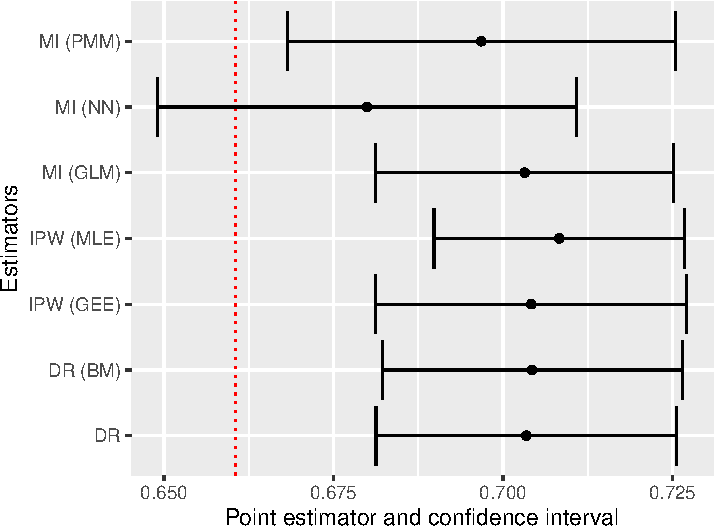
\includegraphics{nonprobsvy-paper_files/figure-latex/comparison of estimates-1} \end{center}

\end{CodeChunk}

\subsection{Advanced usage}\label{advanced-usage}

\subsubsection{Bootstrap Approach for Variance
Estimation}\label{bootstrap-approach-for-variance-estimation}

In each variant, we first draw bootstrap samples based on probability
and non-probability data, and then we perform the appropriate
calculations related to the given estimator to obtain the mean of the
population of the \texttt{l}-th iteration. Finally, we use the usual
formula for the bootstrap variance, and in this way we obtain the
estimate of interest.

The boostrap method is called if its type is defined in the control
argument \texttt{var\_method}, which defaults to \texttt{analytical}.
The number of iterations is set in the \texttt{num\_boot} argument
(default 100).

\begin{CodeChunk}
\begin{CodeInput}
R> est3_logit <- nonprob(
+   selection = ~ region + private + nace + size,
+   target = ~ single_shift,
+   svydesign = jvs_svy,
+   data = admin,
+   method_selection = "logit",
+   control_inference = controlInf(var_method = "bootstrap", num_boot = 50),
+   verbose = F,
+ )
\end{CodeInput}
\end{CodeChunk}

\subsubsection{Variable Selection
Algorithms}\label{variable-selection-algorithms-1}

\begin{CodeChunk}
\begin{CodeInput}
R> est7_glm_sel <- nonprob(
+   outcome = single_shift ~ region + private + nace + size,
+   svydesign = jvs_svy,
+   data = admin,
+   method_outcome = "glm",
+   family_outcome = "binomial",
+   control_outcome = controlOut(nfolds = 5, nlambda = 10),
+   control_inference = controlInf(vars_selection = TRUE),
+   verbose = TRUE
+ )
\end{CodeInput}
\begin{CodeOutput}
Starting CV fold #1
Starting CV fold #2
Starting CV fold #3
Starting CV fold #4
Starting CV fold #5
\end{CodeOutput}
\end{CodeChunk}

\section{Classes and S3methods}\label{classes-and-s3methods}

\section{Summary and future work}\label{summary-and-future-work}

The \pkg{nonprobsvy} package is an R tool developed to address
challenges associated with making inferences from non-probability
samples. As non-probability data sources such as administrative data,
voluntary online panels, and social media data become increasingly
available, statisticians are faced with the problem of how to integrate
these sources with traditional probability samples to produce reliable
population estimates. This package provides a suite of methods
specifically designed to handle the unique characteristics of
non-probability samples, where selection mechanisms are often unknown or
biased.

\pkg{nonprobsvy} supports a range of estimation techniques including
mass imputation, inverse probability weighting (IPW), and doubly robust
(DR) methods. Each of these methods allows researchers to correct for
selection bias in non-probability samples by leveraging auxiliary data
from probability samples or known population totals. The mass imputation
approach imputes values for the outcome variable in the probability
sample using models trained on the non-probability sample. The IPW
estimator uses estimated propensity scores to weight non-probability
samples in a way that aligns them more closely with the population. The
DR estimator combines both approaches, resulting in an estimator that
remains consistent if either the outcome model or the propensity score
model is correctly specified, thus providing a level of robustness
against model misspecification.

Designed to integrate with the widely used \pkg{survey} package in R,
\pkg{nonprobsvy} enables researchers to define survey designs, specify
selection and outcome models, and estimate population parameters using
both probability and non-probability samples. The package supports
advanced modeling options, including generalized linear models, nearest
neighbor algorithms, and predictive mean matching, and allows for
customization of tuning parameters, variable selection, and variance
estimation methods (e.g., bootstrap).

Overall, \pkg{nonprobsvy} is a comprehensive toolkit for researchers and
practitioners working with mixed data sources. It simplifies the
implementation of complex statistical methods for non-probability
samples, making it easier to produce robust, reliable estimates even
when working with non-representative data. By providing a unified
framework for inference with non-probability samples, \pkg{nonprobsvy}
contributes to the growing field of data integration and enhances the
ability of statisticians to make informed decisions from diverse data
sources.

A natural extension of this study is that consistency can be maintained
when the design weights \(d_i\) are replaced by calibration weights,
which is often the case when working with survey sample datasets. In
addition, other methods of estimating propensity scores proposed in the
literature can be considered, such as estimation using the empirical
likelihood approach. It is also worth exploring the situation where the
two probability and non-probability samples overlap, i.e.~there are
units present in both datasets. This type of problem will be the focus
of the author's future work on non--probability sampling, in particular
its integration with other statistical data sources.

\section{Acknowledgements}\label{Acknowledgements}

The authors' work has been financed by the National Science Centre in
Poland, OPUS 20, grant no. 2020/39/B/HS4/00941.

Łukasz Chrostowski is the main author of the package and for the first
draft of the paper. Piotr Chlebicki contributed to the package and
implemented PMM methods. Maciej Beręsewicz was responsible for the
design of the package, small contributions and prepared the final
manuscript.

\clearpage

\appendix

\section{List of symbols}\label{list-of-symbols}

\begin{table}[ht!]
\centering
\begin{tabular}{ll}
\hline
\textbf{Symbol} & \textbf{Description} \\
\hline
$U$ & Target population of size $N$ \\
$N$ & Population size \\
$\boldsymbol{x}_i$ & Vector of auxiliary variables for unit $i$ \\
$y_i$ & Study variable for unit $i$ \\
$S_A$ & Non-probability sample \\
$S_B$ & Probability sample \\
$n_A$ & Size of non-probability sample \\
$n_B$ & Size of probability sample \\
$\pi_i$ & Inclusion probability for unit $i$ in probability sample \\
$d_i$ & Design weight ($1/\pi_i$) for unit $i$ \\
$R_i$ & Indicator of inclusion into non-probability sample \\
$\mu_y$ & Population mean of target variable $Y$ \\
$\pi_i^A$ & Propensity score for unit $i$ in non-probability sample \\
$m(\boldsymbol{x}_i, \boldsymbol{\beta})$ & Regression model for outcome variable \\
$\hat{\mu}_{IPW}$ & Inverse probability weighting estimator \\
$\hat{\mu}_{MI}$ & Mass imputation estimator \\
$\hat{\mu}_{DR}$ & Doubly robust estimator \\
$\boldsymbol{\theta}$ & Parameter vector for selection model \\
$\boldsymbol{\beta}$ & Parameter vector for outcome model \\
$\hat{y}_i$ & Imputed value for unit $i$ \\
$\hat{N}^A$ & Estimated size based on non-probability sample \\
$\hat{N}^B$ & Estimated size based on probability sample \\
\hline
\end{tabular}
\caption{List of symbols and their descriptions}
\label{tab-list-of-sybmols}
\end{table}

\clearpage

\clearpage

\section{Codes for specific methods}\label{sec-examples}

\clearpage

\section{Algorithms}\label{sec-details}

\begin{algorithm}[ht!]
\caption{Mass imputation based on a generalized linear model}
\label{algo-1}
\begin{algorithmic}[1]
 \State Estimate the regression model $\mathbb{E}[Y|\boldsymbol{X}=\boldsymbol{x}]=m(\boldsymbol{x}, \boldsymbol{\beta})$\ basing on units from $S_A$ sample.
 \State For each $i \in S_B$, calculate the imputed value as
 $$
 \hat{y}_i = m\left(\boldsymbol{x}_{i},\hat{\boldsymbol{\beta}}\right).
 $$
\end{algorithmic}
\end{algorithm}

\begin{algorithm}[ht!]
\caption{Mass imputation using the k-nearest-neighbour algorithm}
\label{algo-2}
\begin{algorithmic}[1]
\State If $k=1$, then for each $i \in S_B$ match $\hat{\nu}(i)$ such that
$\displaystyle \hat{\nu}(i)=
\operatornamewithlimits{arg\,min}_{j\in S_{A}}d\left(\boldsymbol{x}_i,\boldsymbol{x}_j\right)$.
\State If $k>1$, then
$$\hat{\nu}(i, z) = \operatornamewithlimits{arg\,min}_{\displaystyle j\in S_{A}\setminus\bigcup_{t=1}^{z-1}
\{\hat{\nu}(i, t)\}} d\left(\boldsymbol{x}_i, \boldsymbol{x}_j\right)$$
i.e. $\hat{\nu}(i, z)$ is $z$-th nearest neighbour from the sample.\;
\State For each $i \in S_B$, calculate the imputed value as
$$
\hat{y}_i = \frac{1}{k}\sum_{t=1}^{k}y_{\hat{\nu}(i, t)}.
$$
\end{algorithmic}
\end{algorithm}

\begin{algorithm}[ht!]
\caption{$\hat{y}-\hat{y}$ Imputation:}
\label{algo-3}
\begin{algorithmic}[1]
\State Estimate regression model $\mathbb{E}[Y|\boldsymbol{X}=\boldsymbol{x}]=m(\boldsymbol{x}, \boldsymbol{\beta})$.\;
\State Impute $$\hat{y}_{i}=m\left(\boldsymbol{x}_{i},\hat{\boldsymbol{\beta}}\right), 
\hat{y}_{j}=m\left(\boldsymbol{x}_{j},\hat{\boldsymbol{\beta}}\right)$$
for $i\in S_{B}, j\in S_{A}$ and assign each 
$i\in S_{B}$ to $\hat{\nu}(i)$, where
$$\displaystyle \hat{\nu}(i)=
\operatornamewithlimits{arg\,min}_{j\in S_{A}}\lVert \hat{y}_{i}-\hat{y}_{j}\rVert$$ or
$$\displaystyle \hat{\nu}(i)=
\operatornamewithlimits{arg\,min}_{j\in S_{A}}d\left(\hat{y}_{i},\hat{y}_{j}\right)$$ if $d$ is not induced by the norm.\;

\State If $k>1$, then:
$$\hat{\nu}(i, z) = \operatornamewithlimits{arg\,min}_{\displaystyle j\in S_{A}\setminus\bigcup_{t=1}^{z-1}
\{\hat{\nu}(i, t)\}} d\left(\hat{y}_{i},\hat{y}_{j}\right)$$
e.g., $\hat{\nu}(i, z)$ is $z$-th nearest neighbor from a sample.\;
\State For $i \in S_B$, calculate imputation value as 
$$
\hat{y}_i = \frac{1}{k}\sum_{t=1}^{k}y_{\hat{\nu}(i, t)}.
$$
\end{algorithmic}
\end{algorithm}

\begin{algorithm}[ht!]
\caption{$\hat{y}-y$ Imputation:}
\label{algo-4}
\begin{algorithmic}[1]
\State Estimate regression $\mathbb{E}[Y|\boldsymbol{X}=\boldsymbol{x}]=m(\boldsymbol{x}, \boldsymbol{\beta})$.\;
\State Impute $\hat{y}_{i}=m\left(\boldsymbol{x}_{i},\hat{\boldsymbol{\beta}}\right)$ 
for $i \in S_{B}$ and assign each 
$i \in S_{B}$ do $\hat{\nu}(i)$, where
$\displaystyle \hat{\nu}(i)=
\operatornamewithlimits{arg\,min}_{j \in S_{A}}\lVert \hat{y}_{i}-y_{j}\rVert$ or
$\displaystyle \hat{\nu}(i)=
\operatornamewithlimits{arg\,min}_{j \in S_{A}}d\left(\hat{y}_{i},y_{j}\right)$ 
if $d$ not induced by the norm.\;
\State If $k>1$, then:
$$\hat{\nu}(i, z) = \operatornamewithlimits{arg\,min}_{\displaystyle j \in S_{A} \setminus \bigcup_{t=1}^{z-1}
\{\hat{\nu}(i, t)\}}
d\left(\hat{y}_{i},y_{j}\right).$$
\State For each $i \in S_B$ calculate imputation value as
$$
\hat{y}_i = \frac{1}{k}\sum_{t=1}^{k}y_{\hat{\nu}(i, t)}.
$$
\end{algorithmic}
\end{algorithm}

\section{Detailed derivations}\label{sec-derivations}

\begin{table}[ht!]
\small
\caption{MLE Functions and Gradients for Different Link Functions}
\centering
\begin{tabular}{p{2cm} p{6.5cm} p{6.5cm}}
\hline
Link & MLE Function & Gradient \\ 
\hline
\code{logit} & 
$\displaystyle
\begin{aligned}
& \sum_{i \in S_{\mathrm{A}}} \boldsymbol{x}_i^{\top} \boldsymbol{\theta} \\
& {} - \sum_{i \in S_{\mathrm{B}}} d_i^{\mathrm{B}} \log \left[ 1 + \exp \left( \boldsymbol{x}_i^{\top} \boldsymbol{\theta} \right) \right]
\end{aligned}
$ & 
$\displaystyle
\begin{aligned}
& \sum_{i \in S_{A}} \boldsymbol{x}_{i} \\
& {} - \sum_{i \in S_{B}} d_{i}^{B} \pi(\boldsymbol{x}_{i}, \boldsymbol{\theta}) \boldsymbol{x}_{i}
\end{aligned}
$ \\ \hline

\code{probit} & 
$\displaystyle
\begin{aligned}
& \sum_{i \in S_{A}} \log \left( \frac{ \Phi( \boldsymbol{x}_{i}^{\top} \boldsymbol{\theta} ) }{ 1 - \Phi( \boldsymbol{x}_{i}^{\top} \boldsymbol{\theta} ) } \right) \\
& {} + \sum_{i \in S_{B}} d_{i}^{B} \log \left[ 1 - \Phi( \boldsymbol{x}_{i}^{\top} \boldsymbol{\theta} ) \right]
\end{aligned}
$ & 
$\displaystyle
\begin{aligned}
& \sum_{i \in S_A} \frac{ \phi( \boldsymbol{x}_i^{\top} \boldsymbol{\theta} ) }{ \Phi( \boldsymbol{x}_i^{\top} \boldsymbol{\theta} ) [ 1 - \Phi( \boldsymbol{x}_i^{\top} \boldsymbol{\theta} ) ] } \boldsymbol{x}_i \\
& {} - \sum_{i \in S_B} d_i^B \frac{ \phi( \boldsymbol{x}_i^{\top} \boldsymbol{\theta} ) }{ 1 - \Phi( \boldsymbol{x}_i^{\top} \boldsymbol{\theta} ) } \boldsymbol{x}_i
\end{aligned}
$ \\ \hline

\code{cloglog} & 
$\displaystyle
\begin{aligned}
& \sum_{i \in S_{A}} \left\{ \log \left[ 1 - \exp \left( -\exp( \boldsymbol{x}_{i}^{\top} \boldsymbol{\theta} ) \right) \right] \right\} \\
& {} + \exp( \boldsymbol{x}_{i}^{\top} \boldsymbol{\theta} ) - \sum_{i \in S_{B}} d_{i}^{B} \exp( \boldsymbol{x}_{i}^{\top} \boldsymbol{\theta} )
\end{aligned}
$ & 
$\displaystyle
\begin{aligned}
& \sum_{i \in S_{A}} \frac{ \exp( \boldsymbol{x}_{i}^{\top} \boldsymbol{\theta} ) \boldsymbol{x}_{i} }{ \pi( \boldsymbol{x}_{i}, \boldsymbol{\theta} ) } \\
& {} - \sum_{i \in S_{B}} d_{i}^{B} \exp( \boldsymbol{x}_{i}^{\top} \boldsymbol{\theta} ) \boldsymbol{x}_{i}
\end{aligned}
$ \\ \hline

\end{tabular}
\end{table}

\bibliography{references.bib}



\end{document}
